\documentclass{article}

\usepackage{enumitem}
\usepackage{geometry}
\usepackage{booktabs}
\usepackage{graphicx}
\usepackage{listings}

\newgeometry{lmargin=3cm, rmargin=3cm, bmargin=2.5cm}
\setlist[itemize]{noitemsep,topsep=-1pt, leftmargin=*}

\title{Description of Data Base}
\author{Krzysztof Piotrowski}
\date{22nd of November}


\begin{document}
\maketitle
\section{Textual description of a database}
\subsection{Aim}
The main aim of this database is to manage travel agency's system.
First of all, it keeps data about transaction between client and company.
Secondly, it covers information about trips in every detail
(including destination, time, place, transport issue and trip's hotel).
Lastly, it is designed to administrate employees' data.
\subsection{Description}
Travel agency offers various types of trip to different countries.
For each trip we store the following: destination, starting and ending dates, price, and maximum number of people that can take part in trip.
Additionally, each trip is associated with information about hotels. Trip can have several hotels and hotels can be associated with different trips, each of that hotel contains information about name, number of stars and exact address location.
Also, trip is associated with transport details, in particular: how client can get to its destination (airplane, bus, etc.) and exact place and time of departure.
Lastly, trip has assigned guide, who is a supervisor of each trip, that take care for each client during their residence. Only one guide is assigned to trip, and each guide can carry on only one trip.
There are two more group of people that database is aware of: clients and agents.
Agents is special type of worker that sell trips to various clients. Company note each transaction and check if client already paid for the trip.
System stores personal details of each person involved in system: they name, surname, mail, telephone number, and address.
Each address consists of a street, street number, zip-code, city, and country. Optinally, It can have apartment number (if occurs).
Each trip, person, hotel, transport detail can be located in system using special numeric ID assigned to each one of them.

\subsection{Objects - entities and attributes}
    \bigskip
    \begin{tabular}{p{.35\textwidth}p{.35\textwidth}p{.35\textwidth}}
        \textbf{Travel Agent} & \textbf{Guide} & \textbf{Customer}\\
        \begin{itemize}
            \item name
            \item surname
            \item mail
            \item telephone
            \item agent ID
        \end{itemize} & \begin{itemize}
            \item name
            \item surname
            \item mail
            \item telephone
            \item guide ID
        \end{itemize} & \begin{itemize}
            \item name
            \item surname
            \item mail
            \item telephone
            \item customer ID
        \end{itemize}\\
    \end{tabular}
    \begin{tabular}{p{.35\textwidth}p{.35\textwidth}p{.35\textwidth}}
        \textbf{Trip} & \textbf{Transport} & \textbf{Hotel}\\
        \begin{itemize}
            \item destination
            \item price
            \item starting date
            \item ending date
            \item max. num. of participants
            \item trip ID 
        \end{itemize} & \begin{itemize}
            \item mean of transport
            \item place
            \item date 
            \item transport ID
        \end{itemize} & \begin{itemize}
            \item name
            \item stars
            \item hotel ID
        \end{itemize}\\
    \end{tabular}
    \begin{tabular}{p{.35\textwidth}p{.35\textwidth}p{.35\textwidth}}
        \textbf{Transaction} & \textbf{Address} & \textbf{City}\\
        \begin{itemize}
            \item payment status
            \item transaction ID
        \end{itemize} & \begin{itemize}
            \item street 
            \item street number
            \item apartment number (optional)
            \item zip code
            \item address ID
        \end{itemize} & \begin{itemize}
            \item country
            \item city
            \item city ID
        \end{itemize}\\
    \end{tabular}
\subsection{Requirements concerning data}
\subsubsection{Data types}
For most of attributes the \textbf{VARCHAR2} will be used sizing from 8 (for zip-code) to 20 (for the rest of attributes).
Numerical values such as telephone, number of stars or IDs will use \textbf{NUMBER} data type. Size will be 8 for IDs, 13 for telephone or 1 for number of stars.
Additionally, there is price which also uses \textbf{NUMBER} but with precision point. Its size is set to 7 digits, where 2 are marked as precision point. 
For any kind of dates, the \textbf{DATE} data type will be used. Also, in database there is one boolean value - it is represented by \textbf{CHAR} data type. 
\subsubsection{Mandatory of attributes}
In this database, almost all of the attributes are mandatory. However, there is one exception - apartment number in address entity is optional.
\newpage
\section{ER Diagram}
\subsection{Diagram}
\begin{figure}[ht]
    \centering{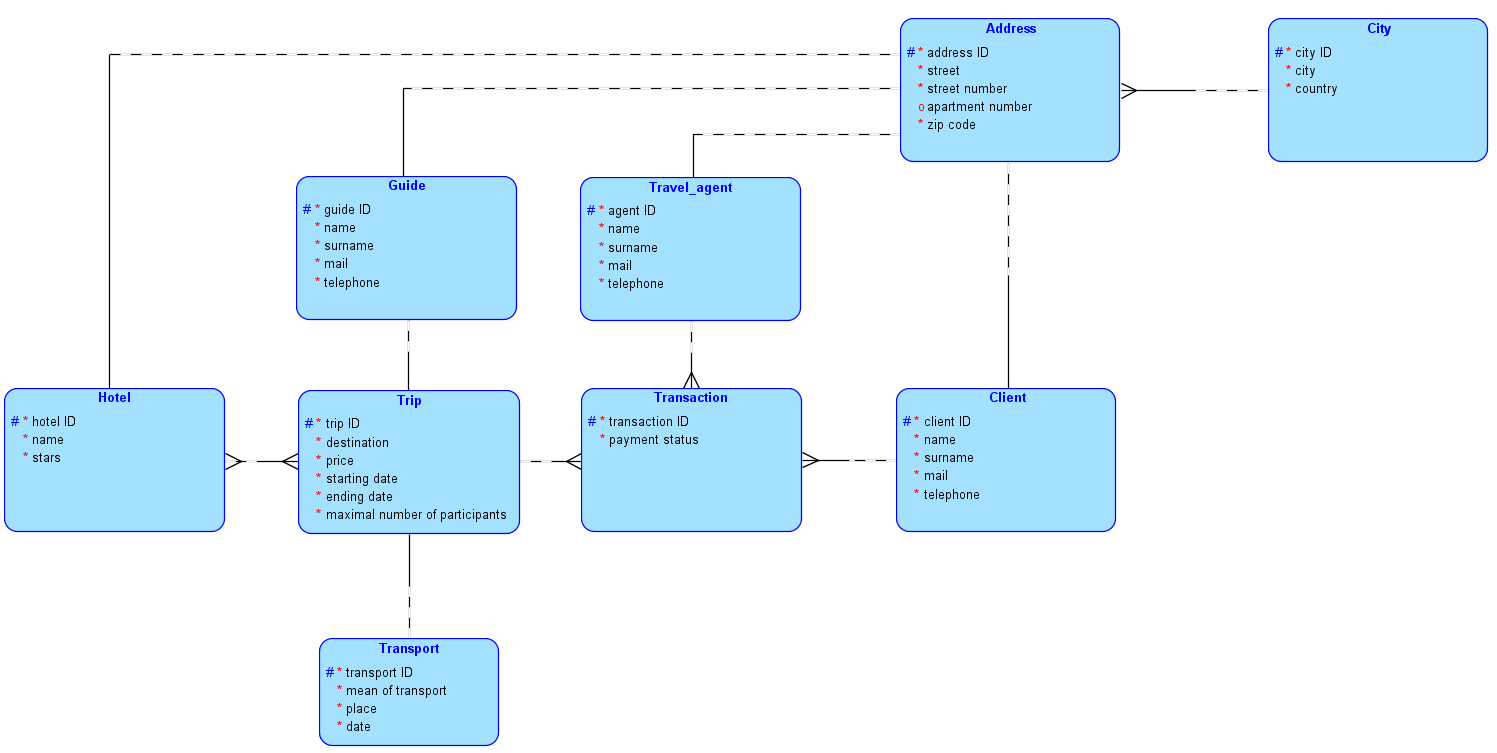
\includegraphics[width=\linewidth]{ER_diagram.PNG}}
\end{figure}
\subsection{Description of entities and their relations}
Each entity will have unique ID to make management easier.
Database has three person entites: travel agent, guide and customer. 
For each of them we store basic information: name, surname and contact details (mail and telephone).
Because address is more complex, it was created as separate entity.
Each person entity is related to address entity.
Address entity stores information about: street, building number and zip code.
It is also related to city entity, which consists of country - city combination, to make the storage easier.
Database connect 3 entities: client, travel agent and trip via transaction entity.
Transaction entity stores information about payment status anda thanks to that it allows client to have more than one trip, trip to have many participants, and travel agent to sell many trips to many clients.
For each trip we store information about price, destination, duration of the trip, maximal number of participants.
Additionally, it is connected with hotel entity.
Hotel entity gathers information about the number of stars and also is related with address entity to know location of a hotel.
Trip can have many hotels (e.g if there is trip around one country) and hotels can have many trips (e.g if there are two different trips to the same location)
Despite connection with hotel or transaction entities, it has obligatory connection with guide entity.
Each trip must have one guide and guide can have zero or one trip.
Additionally, trip must have mandatory relation with transport entity.
Each transport entity covers information about mean of transport, place and date (including time) of departure.

\newpage
\section{Relational Schema}
\subsection{Schema}
\begin{figure}[ht]
    \centering{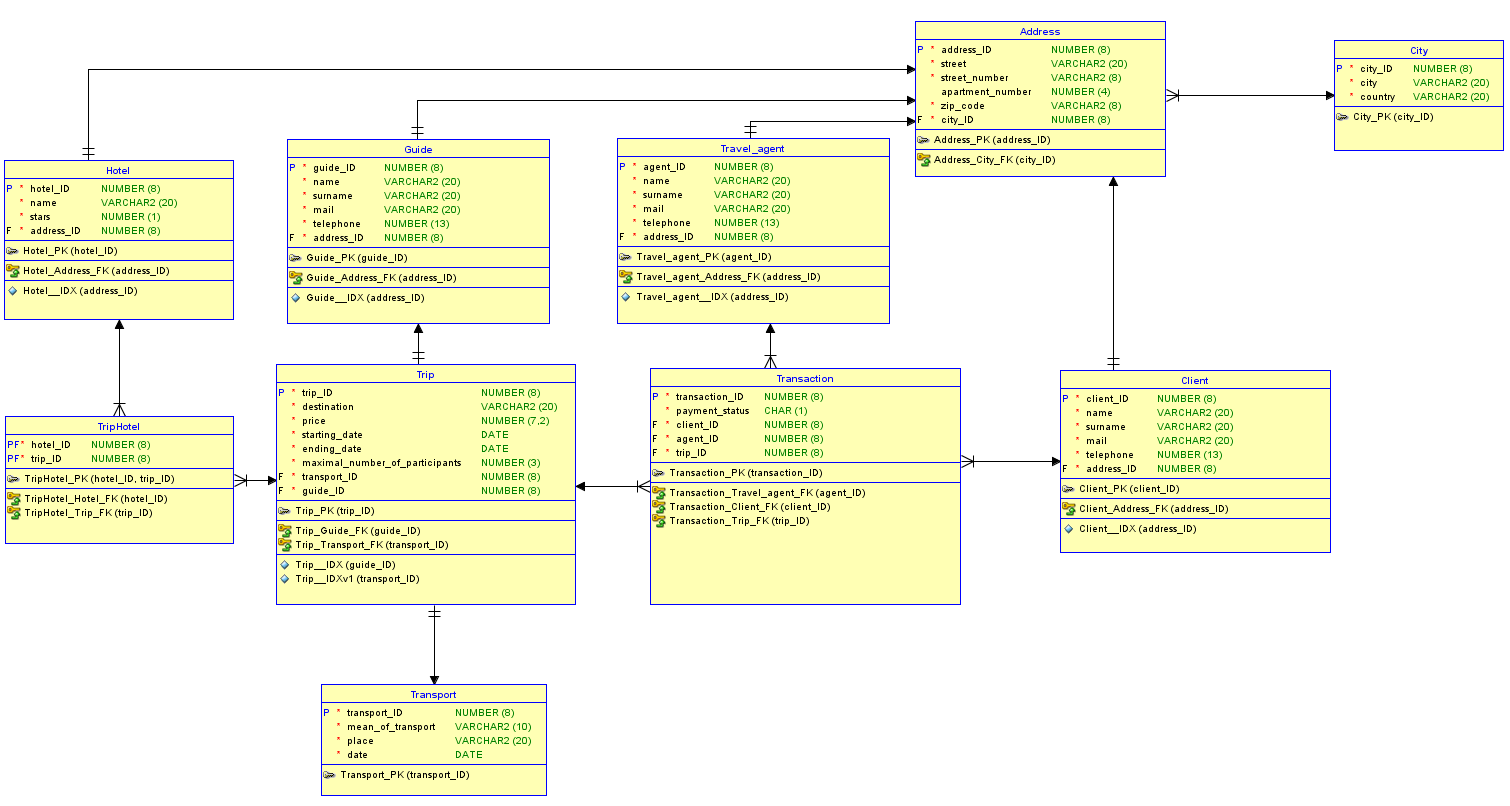
\includegraphics[width=\linewidth]{relational_schema.PNG}}
\end{figure}
\subsection{Description of a way of mapping an ER–diagram into a relational schema}
When all relationships between entities are declared, they must inherit proper keys from other entities as foreign keys.
In my example, each person entity and hotel entity has address ID as foreign key which direct them to their address.
Trip knows his guide ID and transport ID. In transaction entity we have 3 IDs to know who sold, who bought trip and for which trip.
Lastly, address has also city ID to know in which city and country this address occurs.
Because we had special type of relational (M to N) between trip and hotel, new table (sometimes called proxy ) appeared which takes both related entity keys
and change M:N relation into two 1:N relations. It enables trips to have many hotels and hotels to have many trips.

\end{document}

